\documentclass[10pt]{beamer}

  % Math Packages
  \usepackage{amsmath}
  \usepackage{amsthm}
  \usepackage{mathtools}

  % Graphics Packages
  \usepackage{graphicx}
  \usepackage[export]{adjustbox}

  % Colors
  \definecolor{umared}{RGB}{255,74,74}
  \definecolor{mygray}{RGB}{66,66,66}

  % Theme Settings
  \usetheme{metropolis}

  \setbeamercolor{normal text}{fg=mygray}
  \setbeamercolor{alerted text}{fg=umared}
  \setbeamercolor{title text}{fg=mygray}
  \setbeamercolor{title separator}{fg=umared}
  \setbeamercolor{progress bar}{fg=umared}
  \setbeamercolor{frametitle}{bg=umared}

\title{Oracle Taxation Theory}
\logo{
  \makebox[0.13\paperwidth]{\includegraphics[width=1.5cm,keepaspectratio]{Uma_Logo.png} \hfill}
}
\date[]{\today}

\begin{document}

% Title Slide
\begin{frame}
  \titlepage
\end{frame}

% --------------------------------------- %
% Introduction
% --------------------------------------- %
\section{Introduction}

\begin{frame} \frametitle{What do we want to accomplish}

  Questions we are interested in:

  \begin{itemize}
    \item System security\textemdash{Cost of Corruption > Profit from Corruption}
    \item Understand effect of changes in tax rate on equilibrium token price
    \item ?
  \end{itemize}

\end{frame}

\begin{frame} \frametitle{Goals}

  Why economic theory?

  \begin{itemize}
    \item Safe environment for ``testing''
    \item Mathematical formalism makes assumptions transparent
    \item Often learn new things about the environment we build
  \end{itemize}

\end{frame}

% --------------------------------------- %
% Model
% --------------------------------------- %
\section{Model Structure}

\begin{frame} \frametitle{Overview}

  \begin{center}
    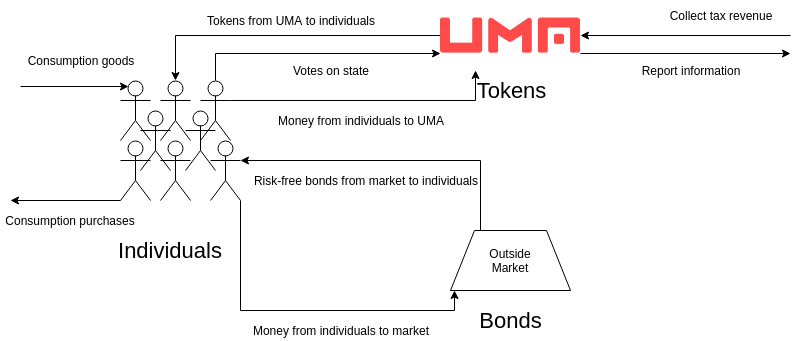
\includegraphics[width=0.8\paperwidth]{ModelOverview.png}
  \end{center}

\end{frame}

\begin{frame} \frametitle{Details: Oracle}

  Must report information to derivatives market, but cannot verify the
  information on its own

  Requires others to vote on information

  Oracle sells voting rights and raises tax revenue ($\mu$ margin taxed at $\tau$)

  Uses revenue to incentivize people to reveal the needed information

\end{frame}

\begin{frame} \frametitle{Details: Individuals}

  There are many individuals

  Each individual likes to eat consumption goods

  Can save for tomorrow using bonds or tokens

\end{frame}

\begin{frame} \frametitle{Details: Voting}

  If an individual owns tokens, they vote on information Oracle must report

  If they choose to tell the truth then

  \begin{itemize}
    \item With probability $\eta$, they forget to vote
    \item With probability $\pi$, they make a mistake
  \end{itemize}

  Liars are deliberate... No forgetting and no mistakes

\end{frame}

\begin{frame} \frametitle{Details: Wealth Evolution}

  All bonds pay return $r$

  Tokens pay depending on what happens:

  If you, and everyone else, attempt to tell truth then

  \begin{align*}
    w_{t+1} &= \begin{cases} (1 + r) b + q x \quad \text{if forget} \\
                             (1 + r) b + (1 + \gamma \frac{\pi}{1 - \pi}) (q + \mu \tau) x \quad \text{if report truth} \\
                             (1 + r) b + (1 - \gamma) (q + \mu \tau) x \quad \text{if mistake} \\
               \end{cases}
  \end{align*}

  If you lie then

  \begin{align*}
    w_{t+1} &= \begin{cases} (1 + r)b + (1 + \gamma \frac{1 - \pi}{\pi})(\mu \tau + {\color{red} 0}) x + {\color{red}\kappa \mu} \quad \text{if corrupted} \\
                             (1 + r)b + (1 - \gamma)(\mu \tau + q) x \quad \text{if not corrupted}
               \end{cases}
  \end{align*}

\end{frame}

% --------------------------------------- %
% Results
% --------------------------------------- %
\section{Results}

\begin{frame} \frametitle{Risk-Neutral Pricing}

  If there were no information or purchasing frictions in a world with risk-neutral
  investors, then all assets would have same return

  \begin{align*}
    (1 + r) &= \frac{\eta q + (1 - \eta) ( (\pi (1 - \gamma) + (1 - \pi) (1 + \gamma \frac{\pi}{1 - \pi})) (\frac{\mu \tau}{n} + q)}{q}
  \end{align*}

  With \$1,000,000 in margin, a 10 basis point tax, and 100,000,000 tokens issued then price per token would be \$

\end{frame}

\end{document}
